% !TEX encoding = UTF-8 Unicode
\documentclass[12pt,a4paper,english
% ,twoside,openright
]{tunithesis}

\special{papersize=210mm,297mm}

\author{Roosa Kuusivaara \& Väinö-Waltteri Granat}
\title{Signal processing in digital holography - Report} % primary title (for front page)
\thesistype{Laboratory Report} % or Bachelor of Science, Laboratory Report...


\usepackage{lastpage}
\usepackage[english]{babel}
\usepackage[
backend=biber,
style=numeric,
citestyle=numeric,
autocite=inline
]{biblatex}
\usepackage{csquotes}
\usepackage{subcaption}
\usepackage{subfigure}
\usepackage{graphicx}

\addbibresource{references.bib} %Imports bibliography file


\definecolor{tunipurple}{RGB}{78, 0, 142}

\newcommand\todo[1]{{\color{red}!!!TODO: #1}} % Remark text in braces appears in red
\newcommand{\angs}{\textsl{\AA}}              % , e.g. slanted symbol for Ångstöm
% Preparatory content ends here


\pagenumbering{roman} % was: {Roman}
\pagestyle{headings}
\begin{document}

% Special trick so that internal macros (denoted with @ in their name)
% can be used outside the cls file (e.g. \@author)
\makeatletter

% Create the title page.
% First the logo. Check its language.
\thispagestyle{empty}
\vspace*{-.5cm}\noindent

\begin{figure}
    \vspace{-1.3cm}
    \advance\leftskip-2.5cm
    \noindent
\includegraphics{img/tunilogo.png}
\end{figure}
 
\vspace{2.5cm}
\begin{flushright}
\noindent\textsf{\LARGE{\@author}}

\noindent\vspace{0.5cm}

\noindent\Huge{\textsf{\textbf{\textcolor{tunipurple}{\@title}}}}
\end{flushright}
\vspace{13.7cm} % adjust to 12.7 this if thesis title needs two lines

% Last some additional info to the bottom-right corner
\begin{flushright}  
    \begin{spacing}{1.0}
      \textsf{Faculty of Information Technology and Communication Sciences (ITC)\\
      \@thesistype\\}
    \end{spacing}
\end{flushright}

% Leave the backside of title page empty in twoside mode
\if@twoside
\clearpage
\fi

% Turn off page numbering for the first pages
\pagenumbering{gobble}


% Some fields in abstract are automated, namely those with \@ (author,
% title, thesis type).
\chapter*{Abstract}
\begin{spacing}{1.0}
\noindent \@author: \@title\\
\@thesistype\\
Tampere University\\
Master’s Degree Programme in Signal Processing\\
November 2023 \\
\end{spacing}
\noindent\rule{12cm}{0.4pt}

\vspace{0.5cm}

% ---------------------------------------
% Abstract and keywords
% ---------------------------------------

\noindent
This report documents the work done in the Signal processing in digital holography assignment as a part of the Advanced signal processing laboratory course. In this assignment we familiarized ourselves with basics of intereference based holography.
~

\noindent\textbf{Keywords:} Hologram, Mach-Zehnder interferometer, Wave propagation.

~


% Add the table of contents


\setcounter{tocdepth}{3}              % How many header level are included
\tableofcontents                      % Create TOC


% The actual text begins here and page numbering changes to 1,2...
% Leave the backside of title empty in twoside mode
\if@twoside
%\newpage
\cleardoublepage
\fi


\renewcommand{\chaptername}{} % This disables the prefix 'Chapter' or
                              % 'Luku' in page headers (in 'twoside'
                              % mode)


\chapter{Introduction}
\label{ch:intro}
In this report we describe our work done in the 'Signal processing in digital holography' laboratory assignment for the Advanced Signal Processing Laboratory course. The work included a hands-on experimentation with a Mach-Zehnder interferometer, which we used to record holographic images. The other section of this lab work is done in Matlab, where we reconstructed the object to 3D from the recorded 2D wavefront data. This report summarizes the methodologies employed and the results obtained in the work. 

\pagenumbering{arabic}
\setcounter{page}{1} 

\chapter{Methodology}
This section describes the methods and equations we used to capture the holograms and reconstruct the objects.

\label{sec:methodology}
\section{Experiment setup}
Holographic imagery relies on the phenomena of light wave superpositions. In this assignment the object is captured using a Mach-Zehnder interferometer, where a monochromatic laser is used to produce two wavefronts. The first wavefront passes trough the object which we want to record, and the second wavefront is used as reference wavefront. The wavefront are the combined to a single wavefront via the interference phenomena, so that one of the wavefronts is combined with the other wavefront in a slight angle, causing a phase difference. The resulting total wave is then captured with a CMOS camera to produce an image file. The phase difference is detectable as fringes in the captured images. The complete setup for the experiment is shown in figure~\ref{fig:lab_setup}.

\begin{figure}
  \centering
  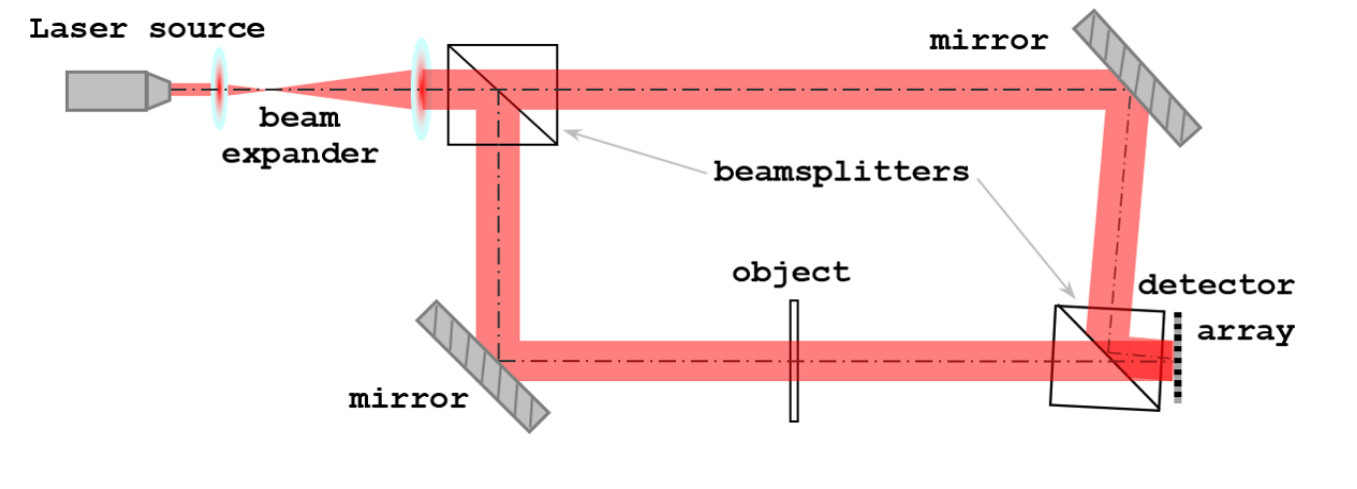
\includegraphics[width=\columnwidth]{img/lab_setup.png}
  \caption{Experiment was done using a Mach-Zehnder interferometer. Taken from~\cite{assignment}}
  \label{fig:lab_setup}
\end{figure}


\section{Object reconstruction}
The object can be extracted from the captured hologram, using a two step method, Fourier filtering and wavefront propagation.

\subsection{Fourier filtering}
First step is to use Fourier filtering to extract the object wave. Since we know that the hologram is defined by the following equation:
\begin{equation}
H(x, y) = E_0(x, y)^2 + E_r(x, y)^2 + U_0(x, y)U_r^*(x, y) + U_0^*(x, y)U_r(x, y)
\label{eq:hologram}
\end{equation}

Where $H(x,y)$ is the hologram wavefront in given position, $E_0$ is the objects amplitude, $E_r$ is the reference wave's amplitude, $U_r$ is the reference wavefront and $U_0$ is the object wavefront which we want to extract. The extraction can the be accomplished by performing frequency filtering to the Fourier transformation of the hologram, which is shown in equation~\ref{eq:hologramfft}. From the Fourier transformation we can see that the second term of the hologram contains the object wavefront $U_0$. Equations~\ref{eq:secondterm} and~\ref{eq:thirdterm} show the Fourier transformations for the second and third term respectively.

\begin{align}
\mathcal{F}[H(x, y)] &= \mathcal{F}\left[E_0(x, y)^2 + E_r(x, y)^2\right] + \mathcal{F}\left[U_0(x, y)E_r \exp(i2\pi\eta)\right] \notag \\
& + \mathcal{F}\left[U_0^*(x, y)E_r \exp(-i2\pi\eta)\right]
\label{eq:hologramfft}
\end{align}

\begin{equation}
F [U_0(x, y)E_r \exp(i2\pi\eta)] = F [U_0] E_r \otimes \delta(f - \eta)
\label{eq:secondterm}
\end{equation}

\begin{equation}
F [U_0^*(x, y)E_r \exp(-i2\pi\eta)] = F [U_0^*] E_r \otimes \delta(f + \eta)
\label{eq:thirdterm}
\end{equation}

By removing all the other terms from the Fourier transformation of the hologram, we are left with only the Fourier transformation of the object wave. The object wave can the be brought back to spatial domain with inverse Fourier transformation. The figure~\ref{fig:fourierfiltering} shows how the second term is isolated from the rest of the hologram.

\begin{figure}
  \centering
  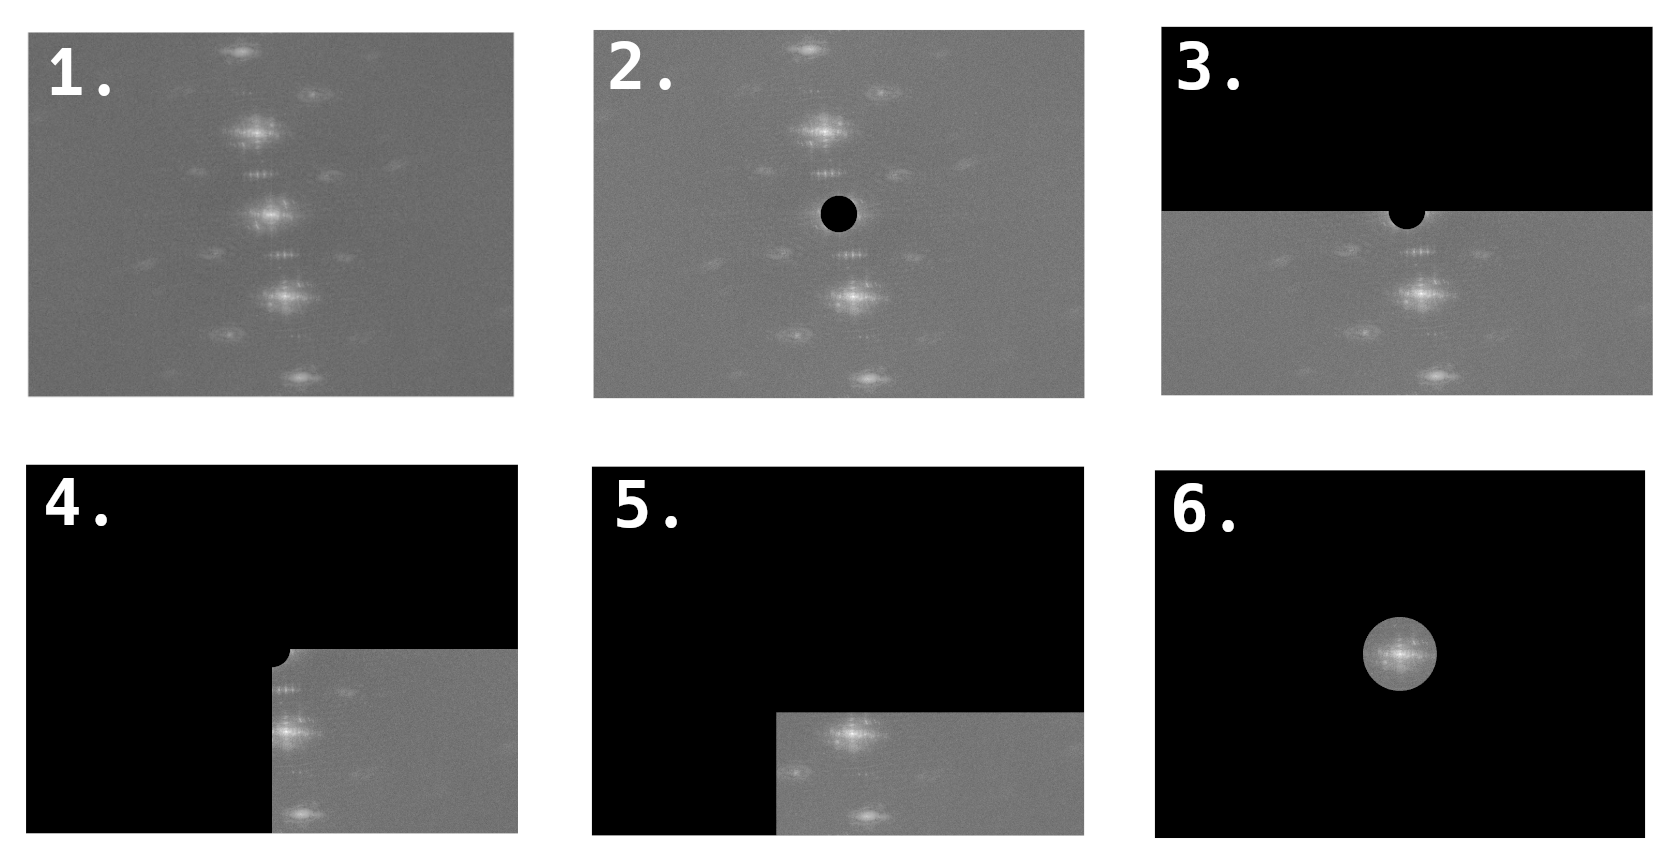
\includegraphics[width=\columnwidth]{img/filter_process.png}
  \caption{Extracting the second term from Fourier transformation of the hologram}
  \label{fig:fourierfiltering}
\end{figure}

\subsection{Wave propagation}
The wavefront alone isn't that usable. The object needs to be projected to an object plane using wave propagation. Using Rayleigh-Sommerfield holographic model with the angular spectrum transfer function defined in equation~\ref{eq:transferfunction} the object is projected on the object plane as defined by the equation~\ref{eq:projection}, where $z$ is the propagation distance. 

\begin{align}
H(f_x,f_y,z) &=
\begin{cases}
\exp[i2\pi z \sqrt{1 - \lambda^2 (f_x^2 + f_y^2)}],& f_x^2 + f_y^2 \leq 1/\lambda^2 \\
0, & \text{otherwise}
\end{cases} \label{eq:transferfunction}
\end{align}

\begin{align}
U_0(x,y,z) &= F^{-1}[H(f_x,f_y,z) \cdot F[U_0(x,y,0)]] \notag \\
\label{eq:projection}
\end{align}
To reconstruct an object that is in focus, we need to determine the optimal distance for the wave to be propagated. This can be accomplished with an autofocusing algorithm or manually by comparing reconstruction results with different values of $z$ by eye.

\chapter{Results}
\label{sec:results}
This section of report presents the results of the wavefront reconstruction, analysis of those results and discusses possible sources of errors in our results. The object wavefront reconstruction process described in the section~\ref{sec:methodology} was implemented as a Matlab script, using a provided implementation of the wave propagation algorithm. 

\section{Wavefront Reconstruction}
In the laboratory we captured to hologram containing the same object with two different fringe widths. The distance between ray and camera was 11 cm, wavelength was ${532 * 10^{-9}}$ m, and a number of pixels was ${3,45*10^{-6}}$ m. The first hologram had fringes of 5 pixels and the second had fringes of 12 pixels. The figures~\ref{fig:5px} and~\ref{fig:12px} show the amplitude and phase images of the reconstructed object wavefronts. 
To determine the optimal propagation distance ($z$) for our figures, we implemented a "slider" to dynamically adjust the distance value. With this tool, we fine-tuned the reconstruction to get the sharpest phase image. In 5 pixel fringe hologram, the best propagation distance was 29,77 cm. In 12 pixel fringe hologram, the sharpest details of phase was determined to be 29,86 cm.

\begin{figure}
  \centering
  \subfigure[Amplitude]{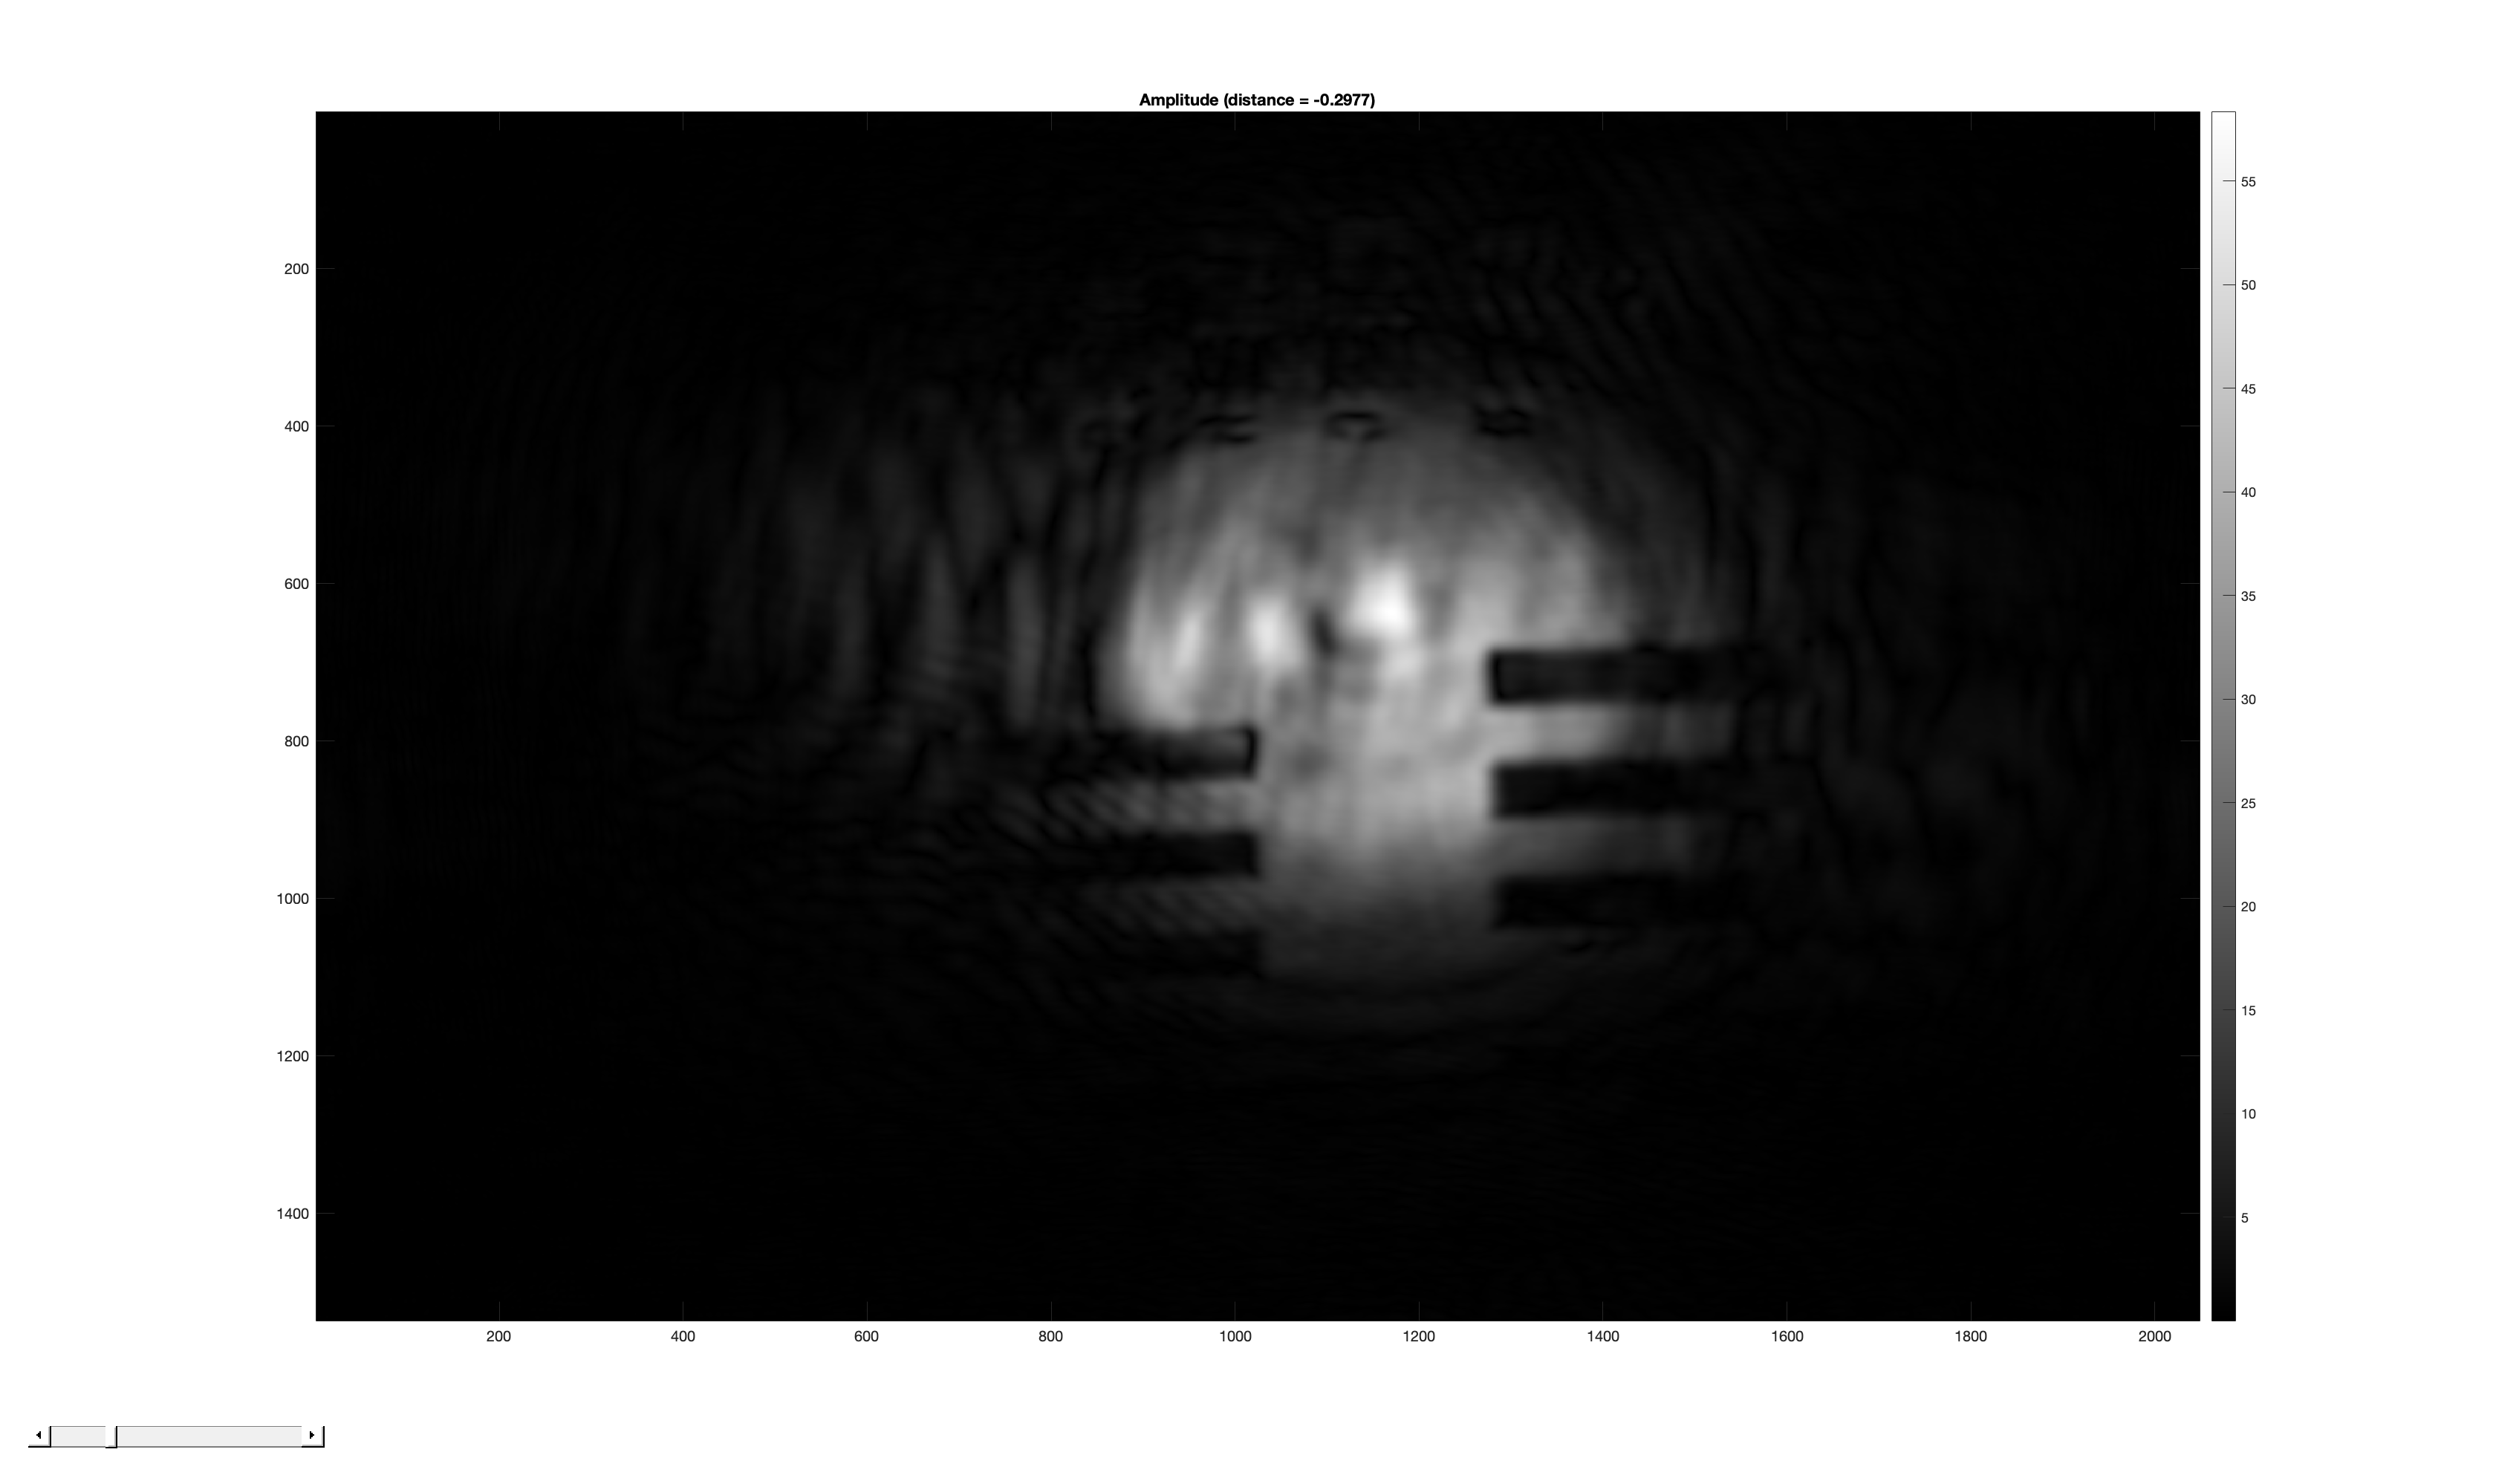
\includegraphics[width=0.49\linewidth]{img/5px_amplitude.png}}
  \subfigure[Phase]{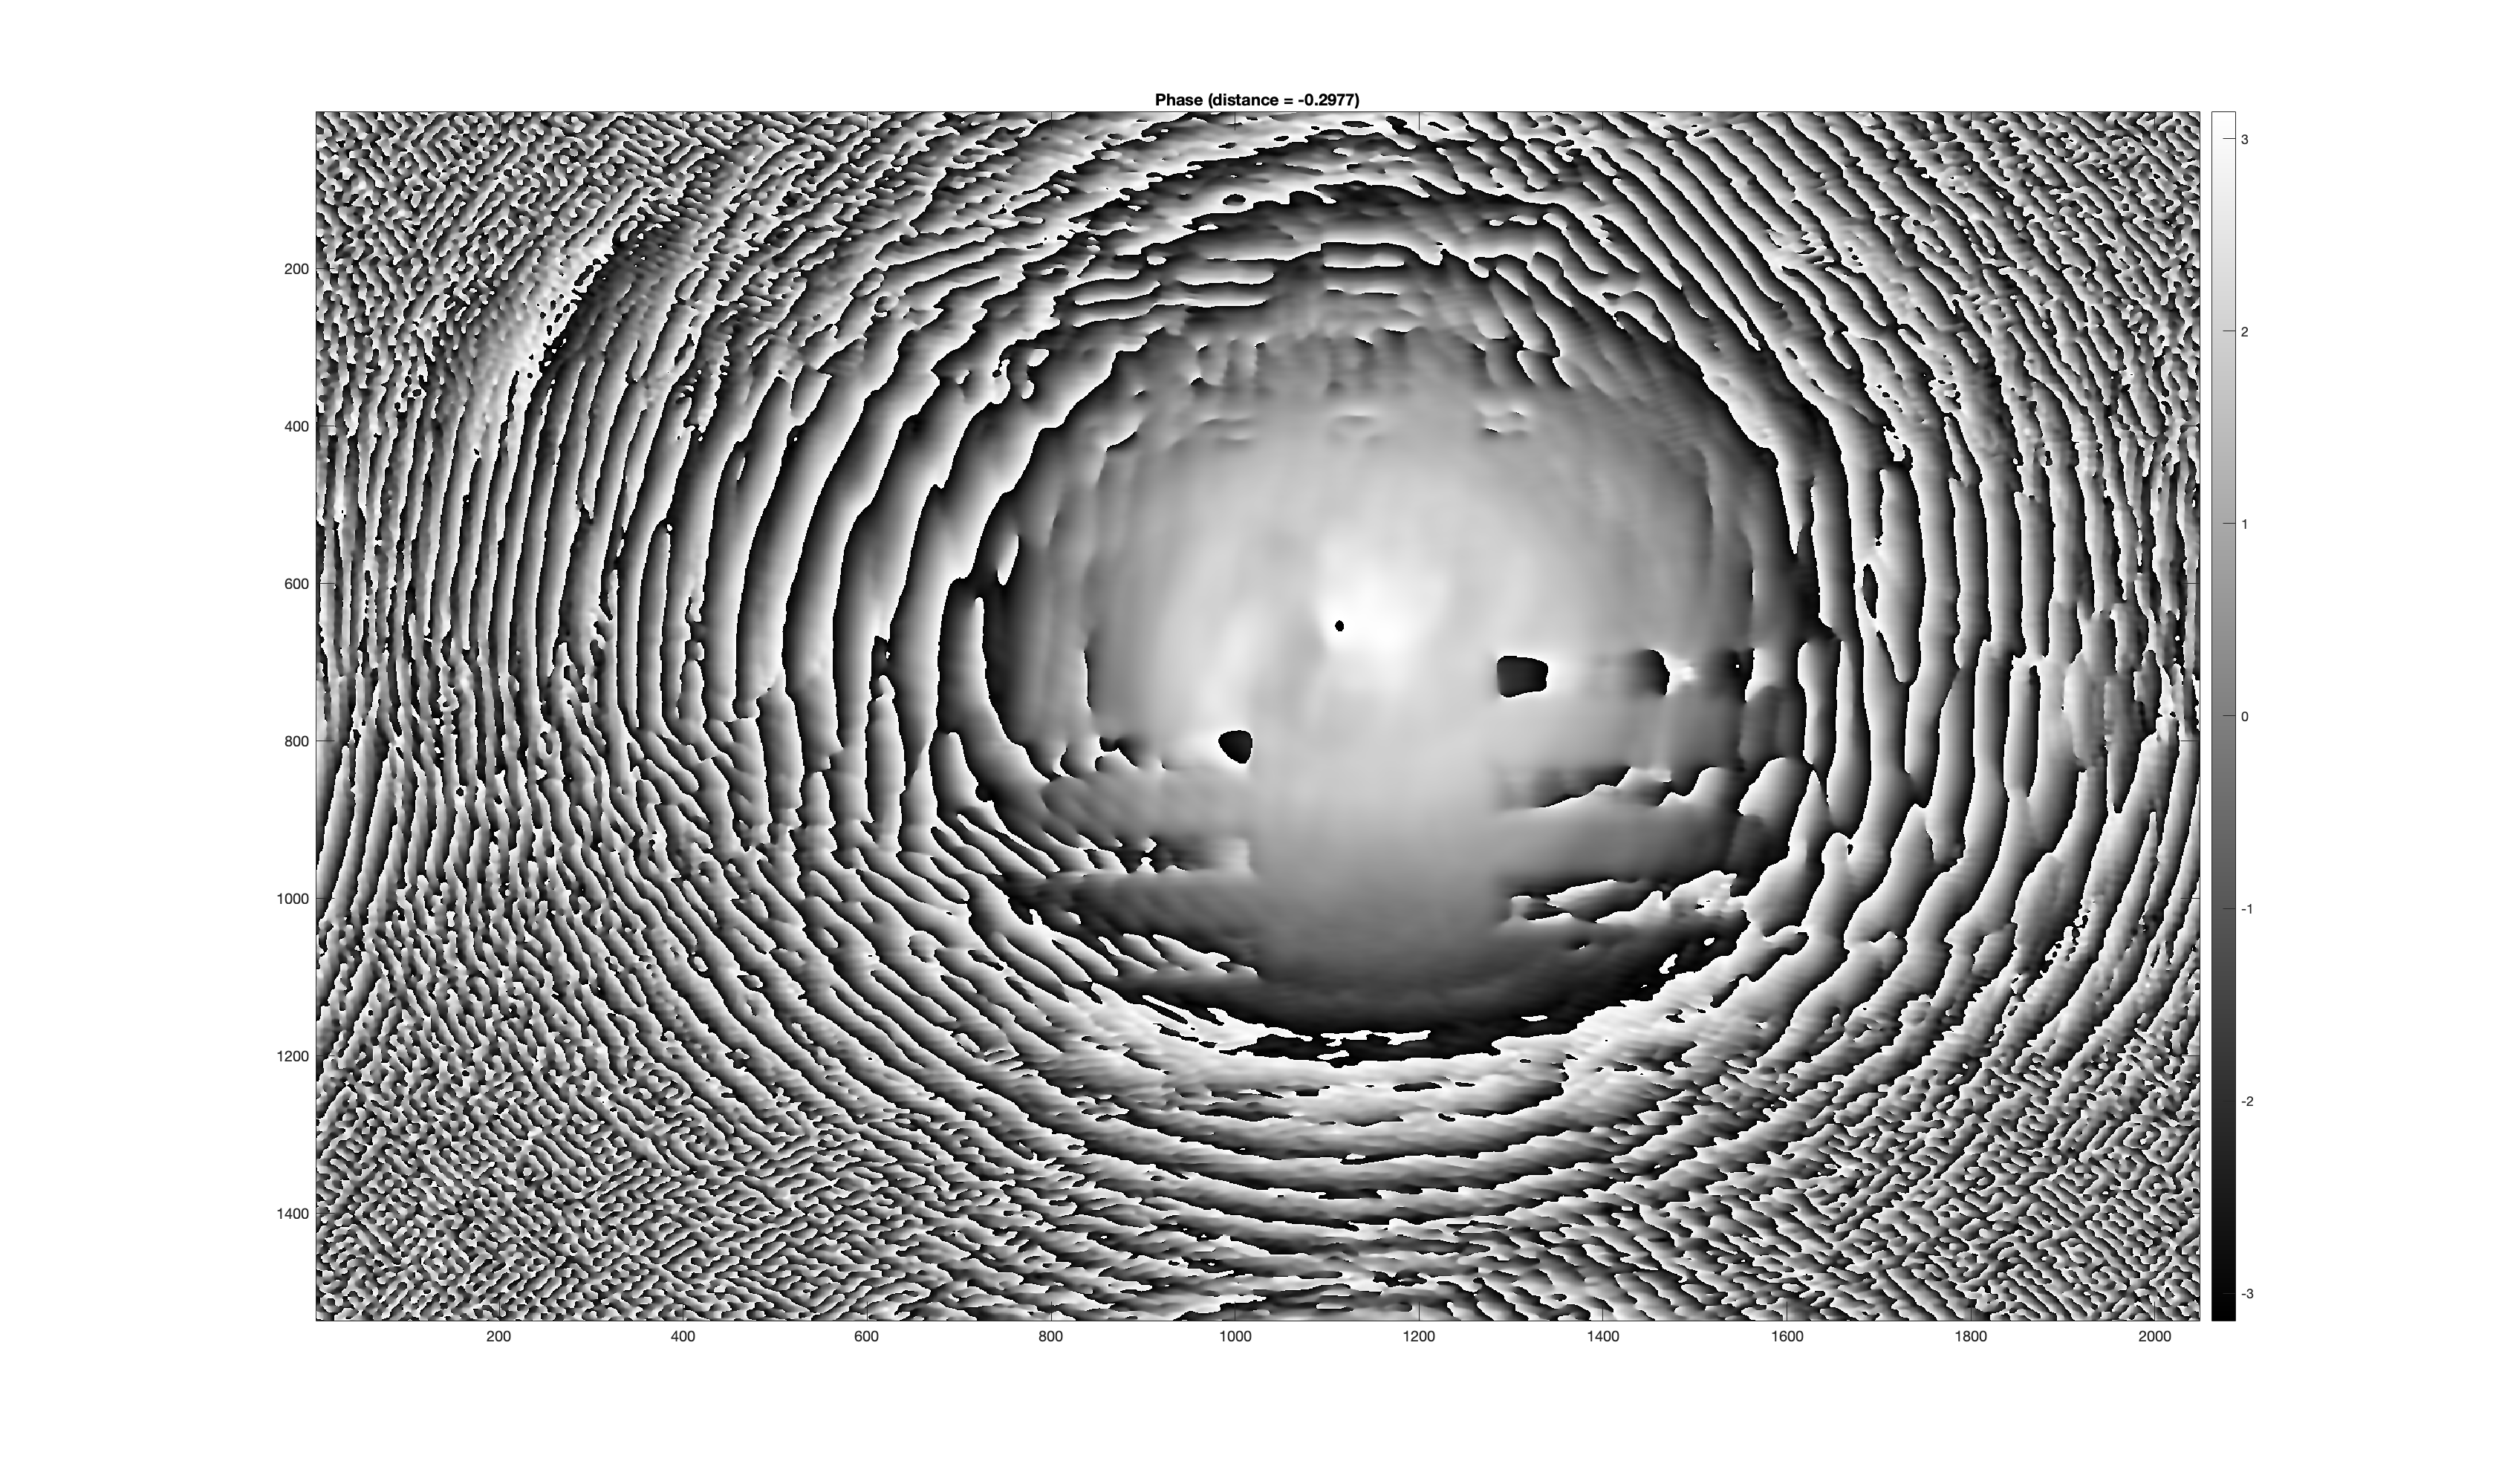
\includegraphics[width=0.49\linewidth]{img/5px_phase.png}}
  \caption{Object wavefront reconstruction of the 5px fringe image}
   \label{fig:5px}
\end{figure}


\begin{figure}
  \centering
  \subfigure[Amplitude]{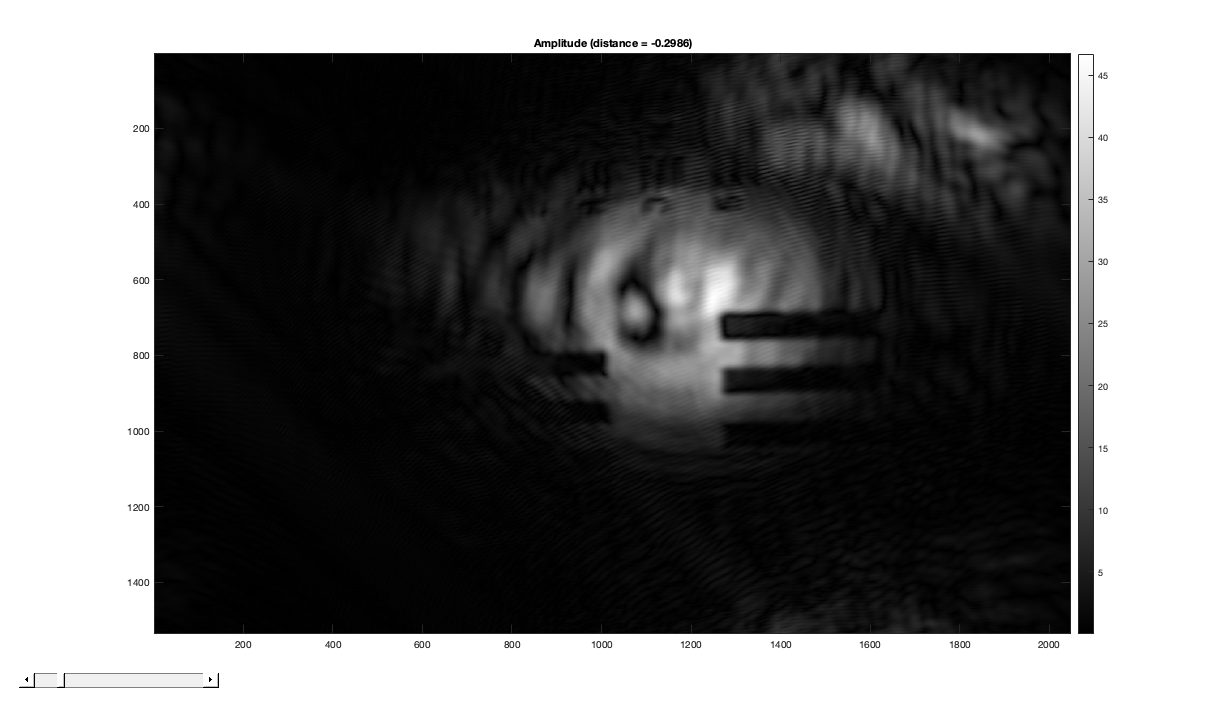
\includegraphics[width=0.49\linewidth]{img/12px_amplitude.png}}
  \subfigure[Phase]{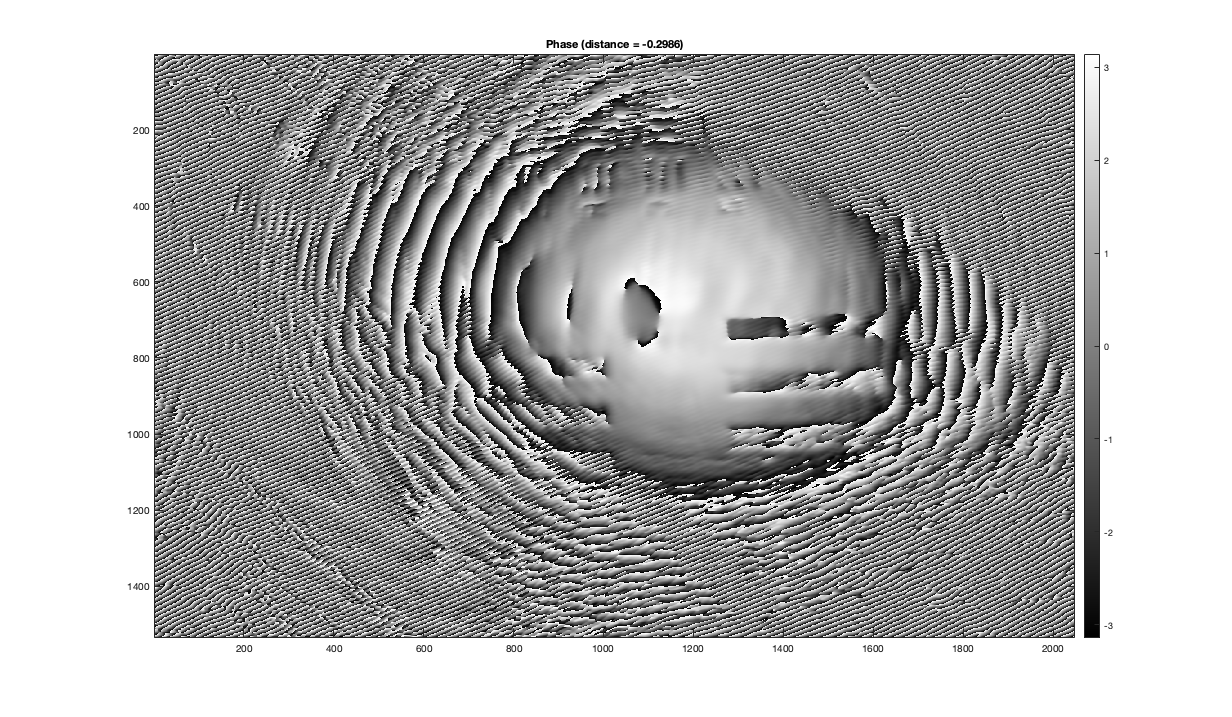
\includegraphics[width=0.49\linewidth]{img/12px_phase.png}}
  \caption{Object wavefront reconstruction of the 12px fringe image}
    \label{fig:12px}
\end{figure}

\section{Analysis}
From the images we can see that the picture with smaller fringes had a more clear reconstruction, and the image with larger fringes was more blurry even after fine tuning the focus. This is because the smaller fringes enable for finer phase information to be captured. This is how higher resolution cameras can capture more information than lower resolution cameras, creating sharper images when capturing objects in focus.

Figure~\ref{fig:lines} compares the mean amplitudes and phases of between the two captured object wavefronts. From the figure we can see that wavefront with 5px fringes has noticeable higher amplitude along the part of the image where the object is. This indicates that more light is present at that part in comparison to the image with 12px fringes. In an image with 12px fringes, a low amplitude indicates a decrease in spatial frequency. This reduced spatial frequency results in a reduced ability to capture and present variations in light, resulting in a loss of detail in the holographic reconstruction. ~\cite{holography}

The phase comparison doesn't tell more than that the wavefronts are in different phases. This makes sense since the angle of the mirrors is different between the images, causing interference in different phase.

\section{Sources of errors}
Several potential sources of errors may impact the accuracy of our laboratory work. First of all, there could be some errors with the laboratory equipments and setup. For example misalignment of optical components, camera calibration, laser stability or inaccurate angle adjustment. Also human factors, external noise or interference during the hologram capturing can affect to the quality of the holograms. Mistakes in the code for wavefront reconstruction may introduce errors, and also incorrectly focusing the optimal propagation distance of the object. In this work, the distance is only focused by eye.

\begin{figure}
  \centering
  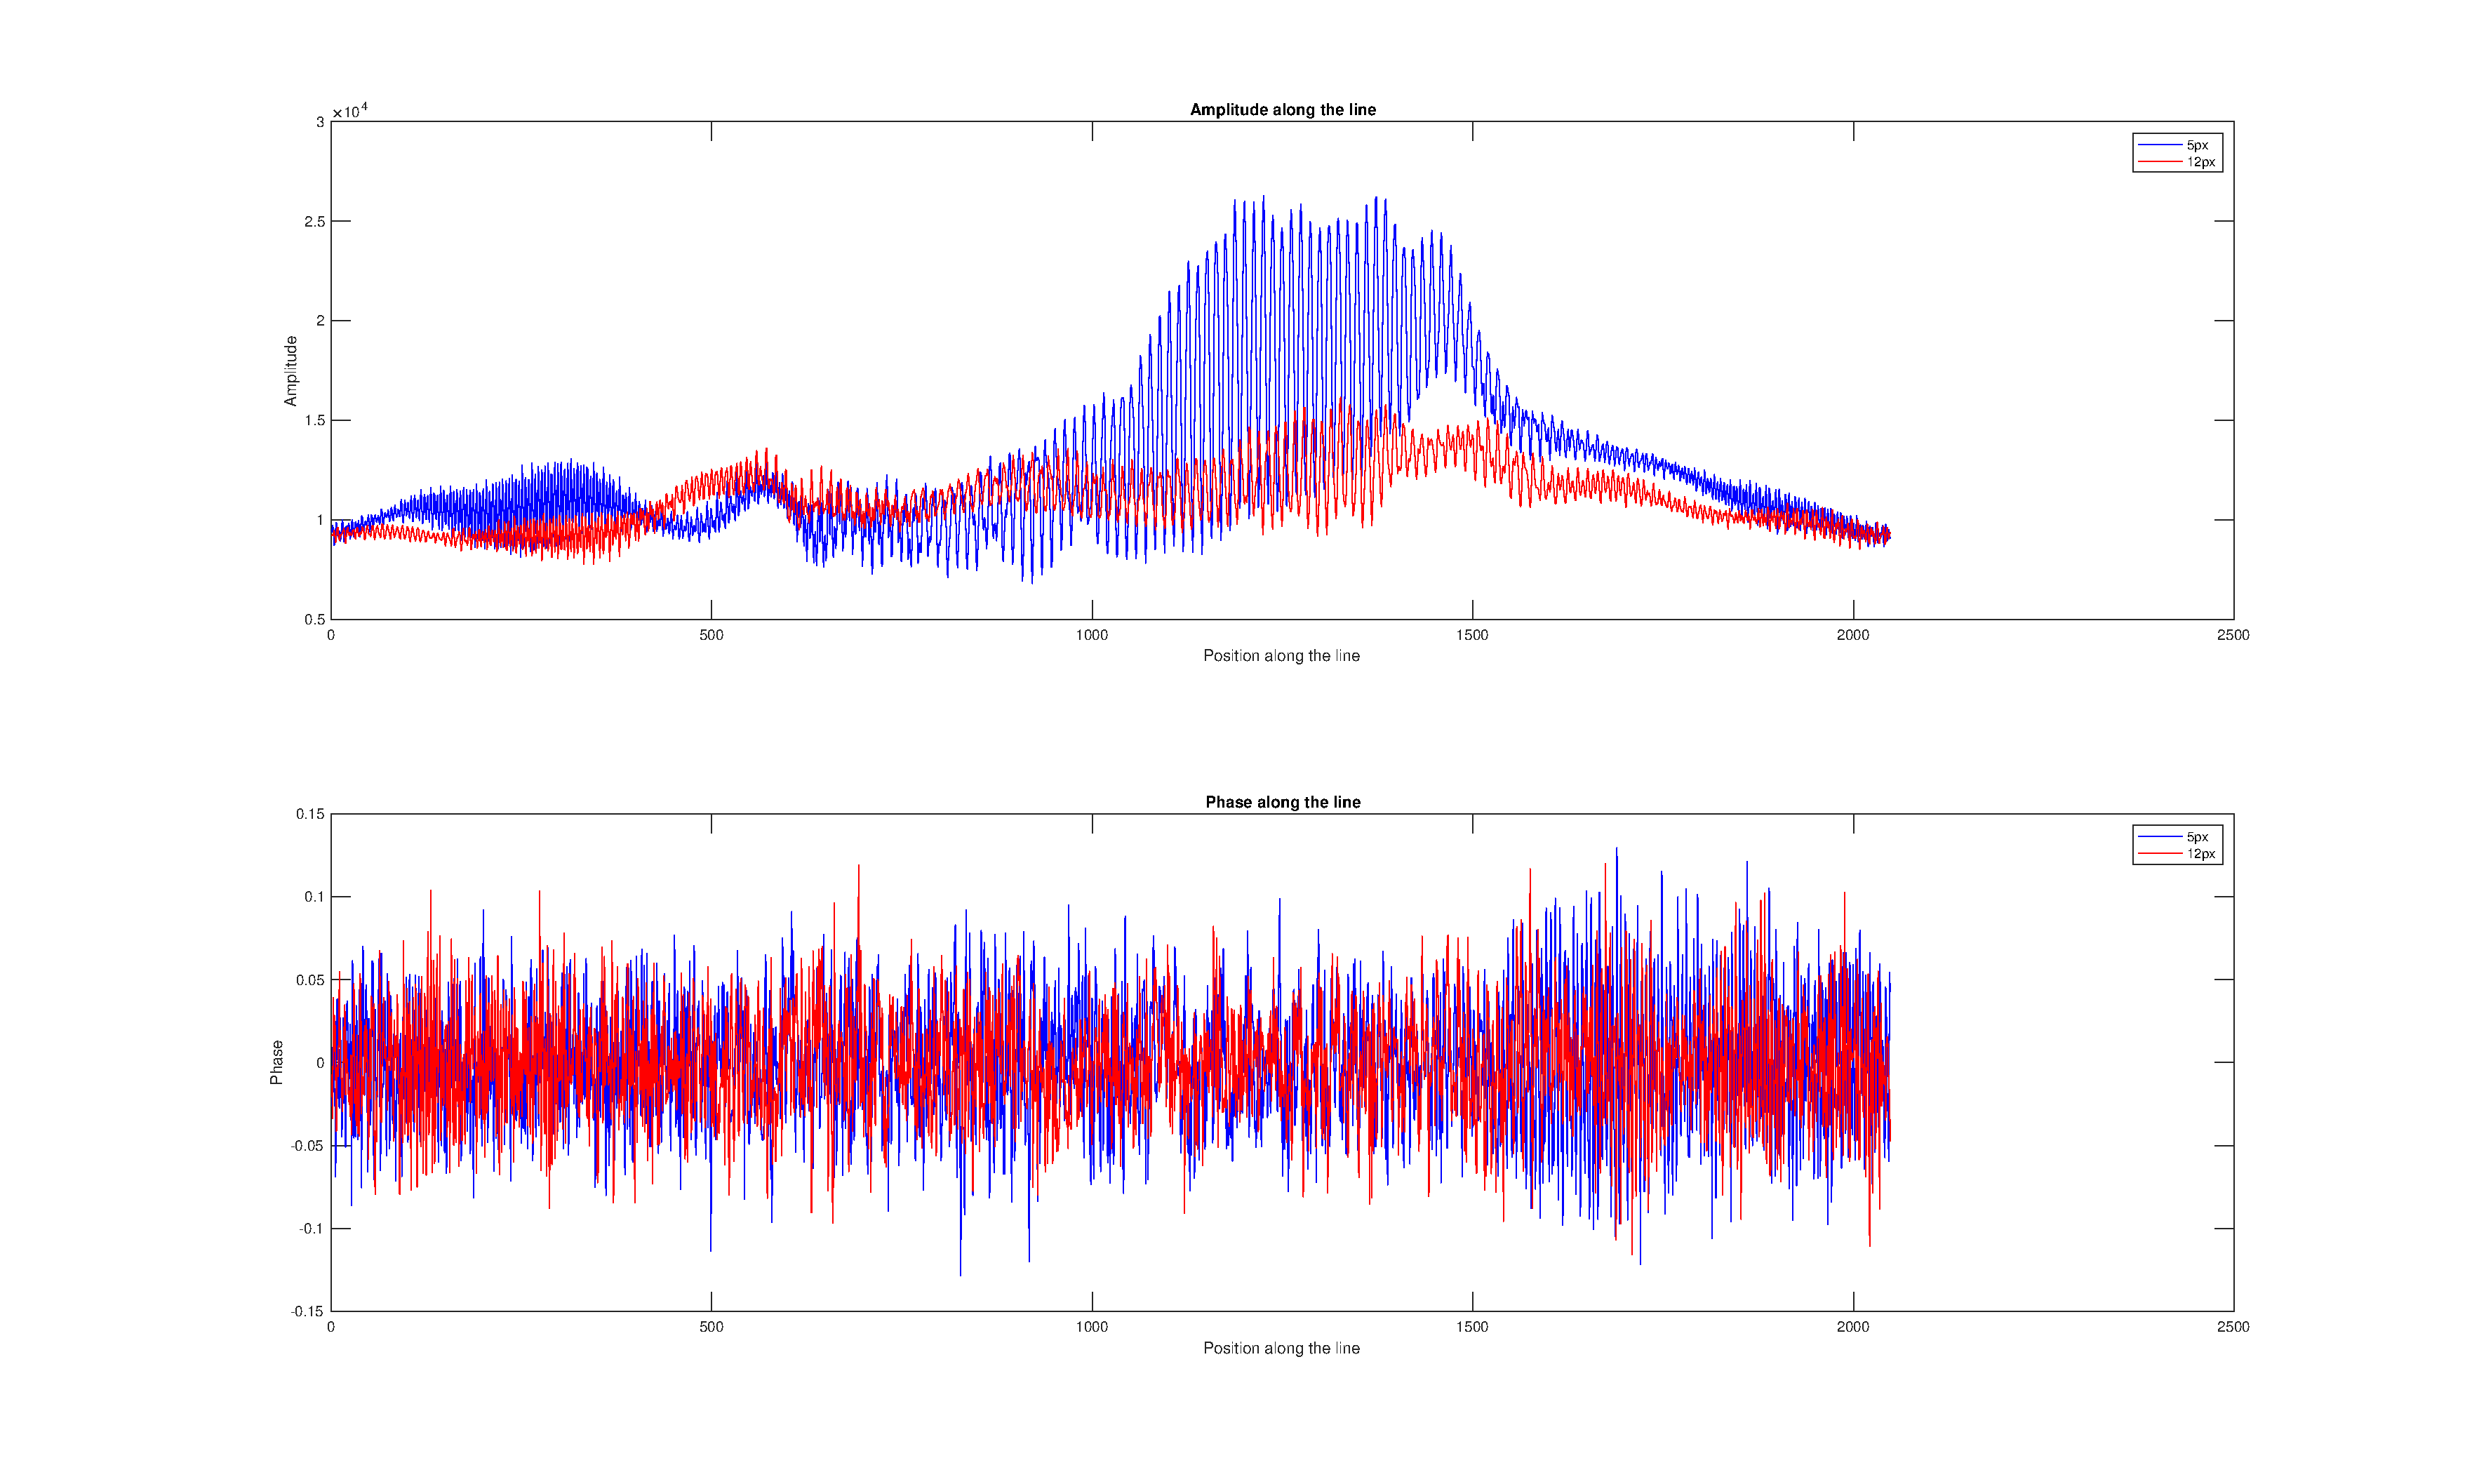
\includegraphics[width=\columnwidth]{img/lines.eps}
  \caption{Amplitude and phase graphs for objects with 5px and 12px fringes}
  \label{fig:lines}
\end{figure}



\chapter{Conclusions}
\label{ch:conclusions}
The goal of this assignment was to learn about signal processing in digital holography by capturing and reconstructing an object from a holographic image, by methods of Fourier filtering and wave propagation. The hologram was created and captured with a Mach-Zehnder interferometer, and the reconstruction was successfully implemented with a Matlab script.
From the reconstruction results we were able to concluded that using a smaller angle between that wavefront produces smaller fringes, which in turned allowed for better reconstruction of the captured objects.


%
% The bibliography, i.e the list of references
%
\newpage

\printbibliography[title=References]
\addcontentsline{toc}{chapter}{References}
\appendix
\pagestyle{headings}

%
% a) Not-so-handy way, but at least it works
%
\def\appA{APPENDIX} % Define the name and numbering manually
\chapter*{\appA}                       % Create chapter heading
\markboth{\appA}{\appA}                % Set page header
\addcontentsline{toc}{chapter}{\appA}  % Include this in TOC
% Note that \label does not work with unnumbered chapter
\begin{figure}[p]
    \centering
    \rotatebox{270}{
        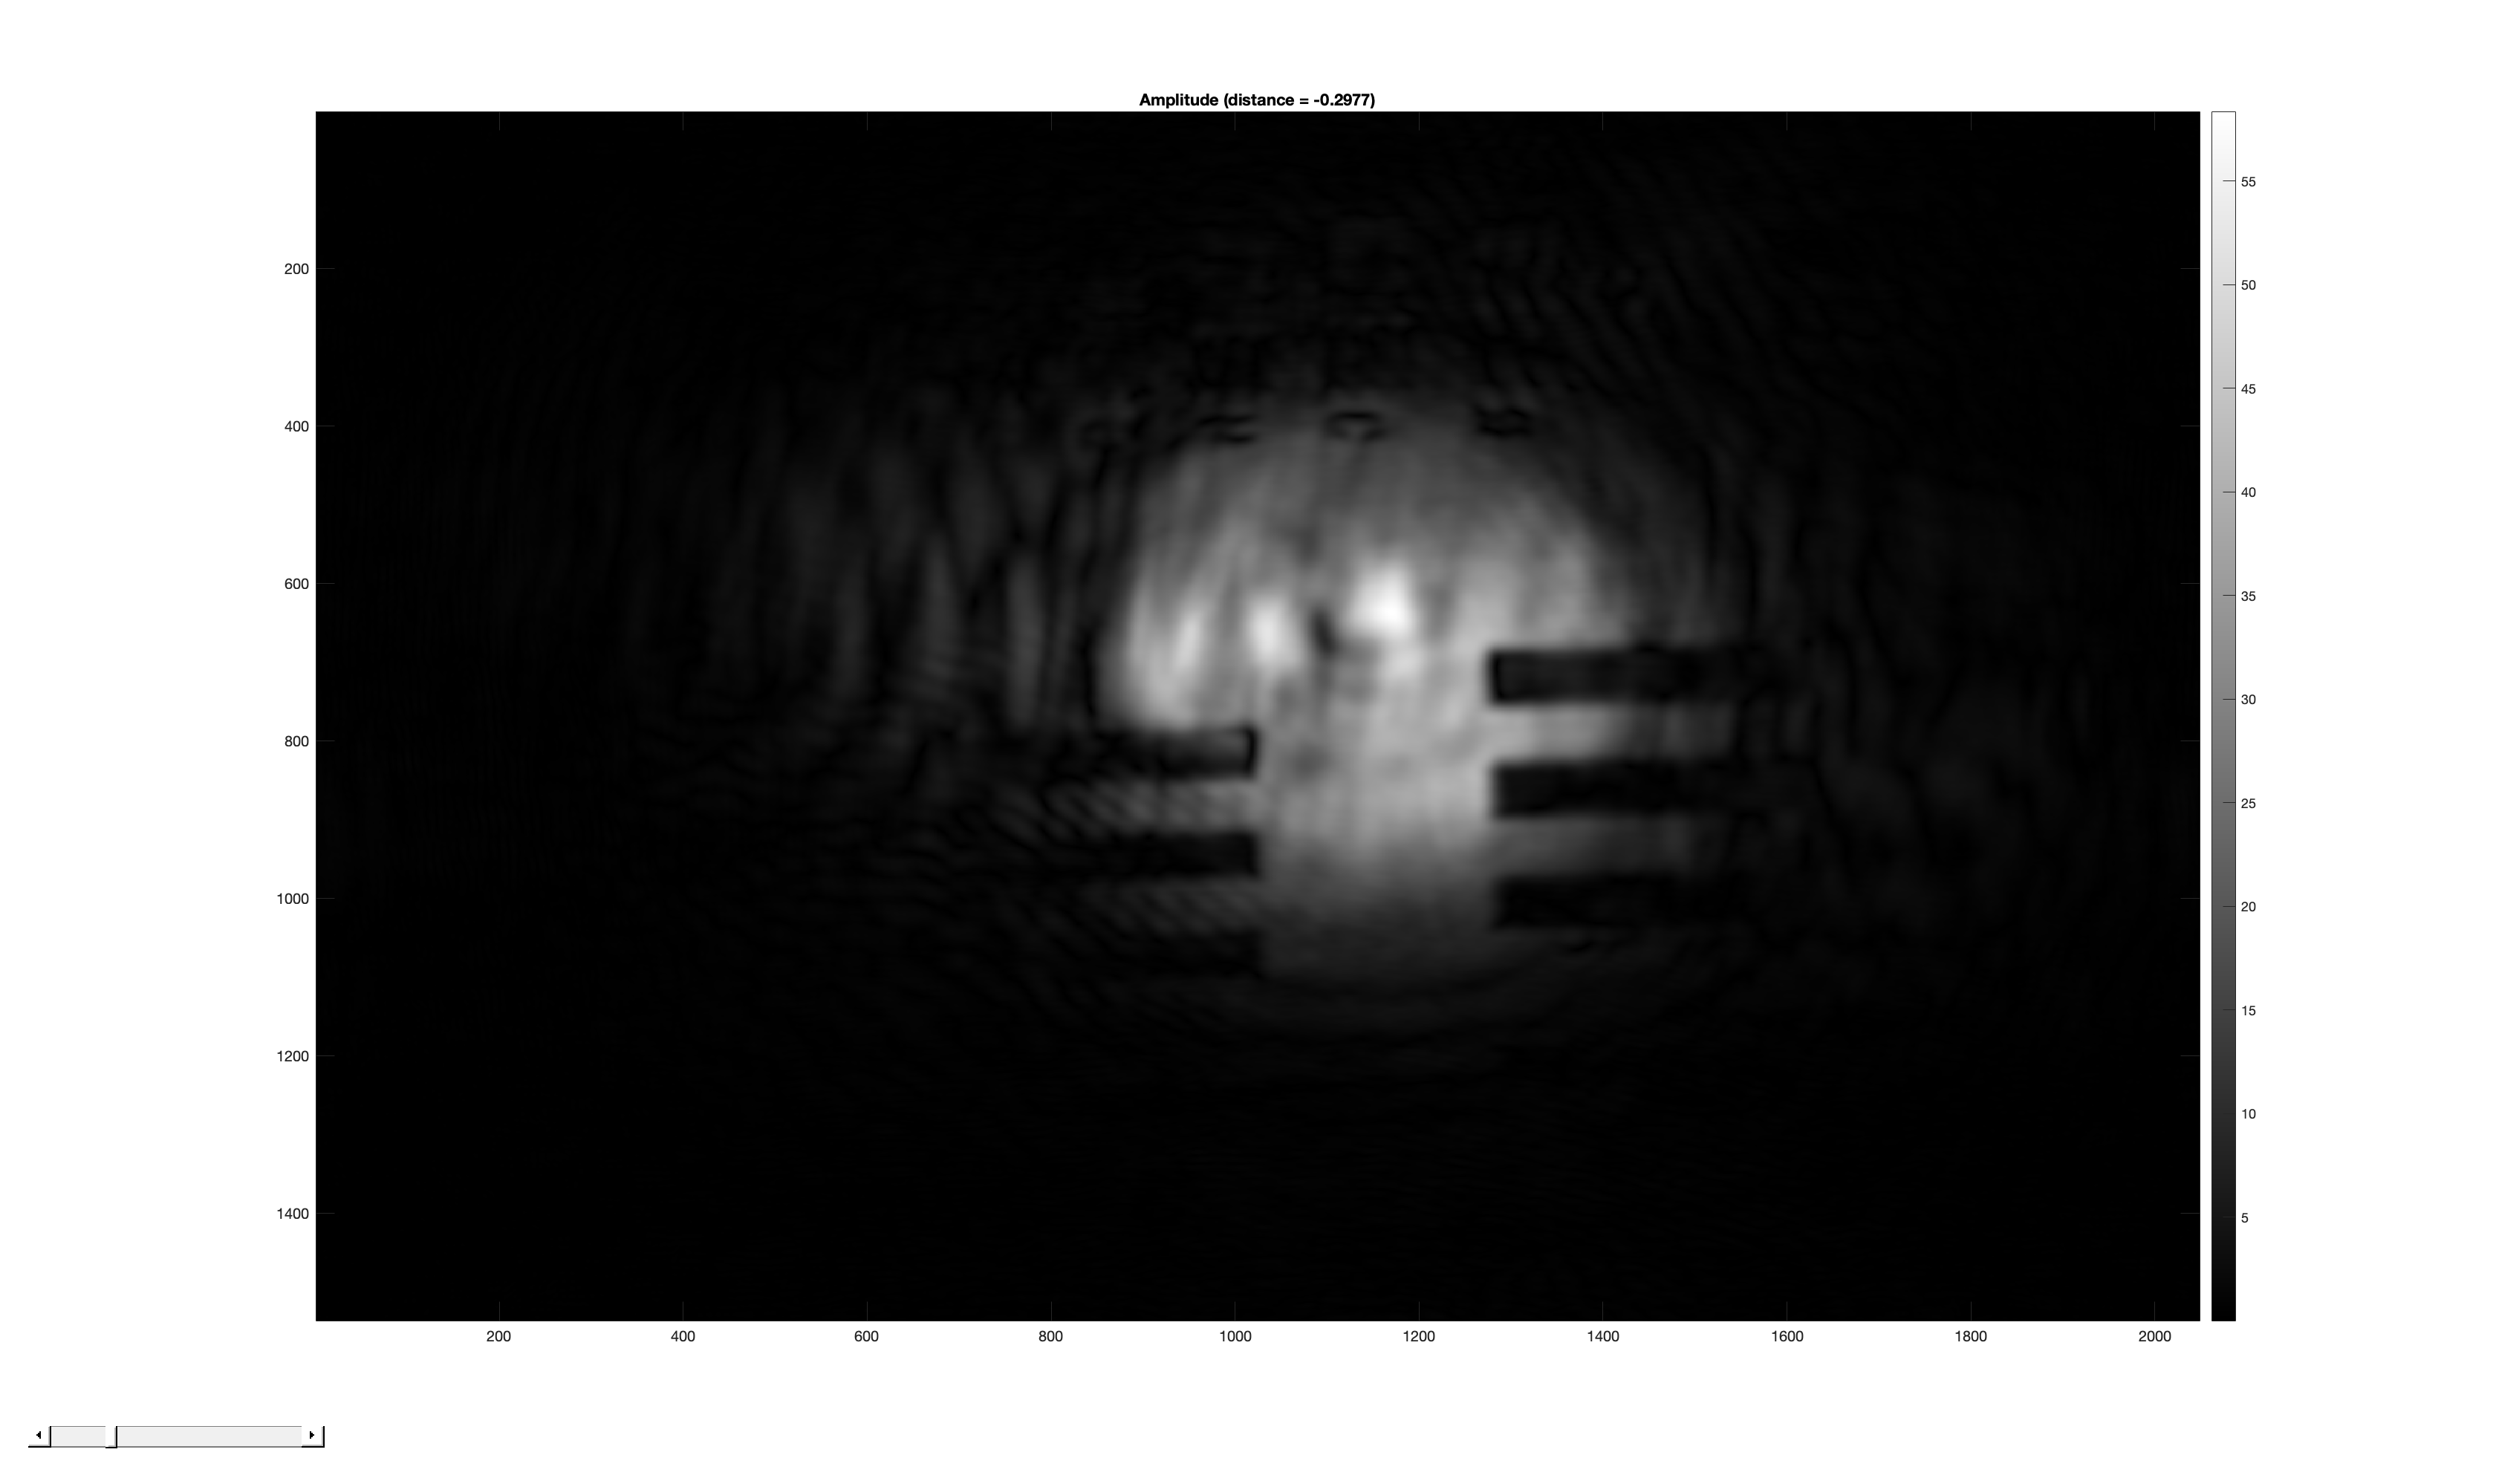
\includegraphics[width=\textheight]{img/5px_amplitude.png}
    }
    \caption{Amplitude of 5px image}
    \label{fig:my_label}
\end{figure}

\begin{figure}[p]
    \centering
    \rotatebox{270}{
        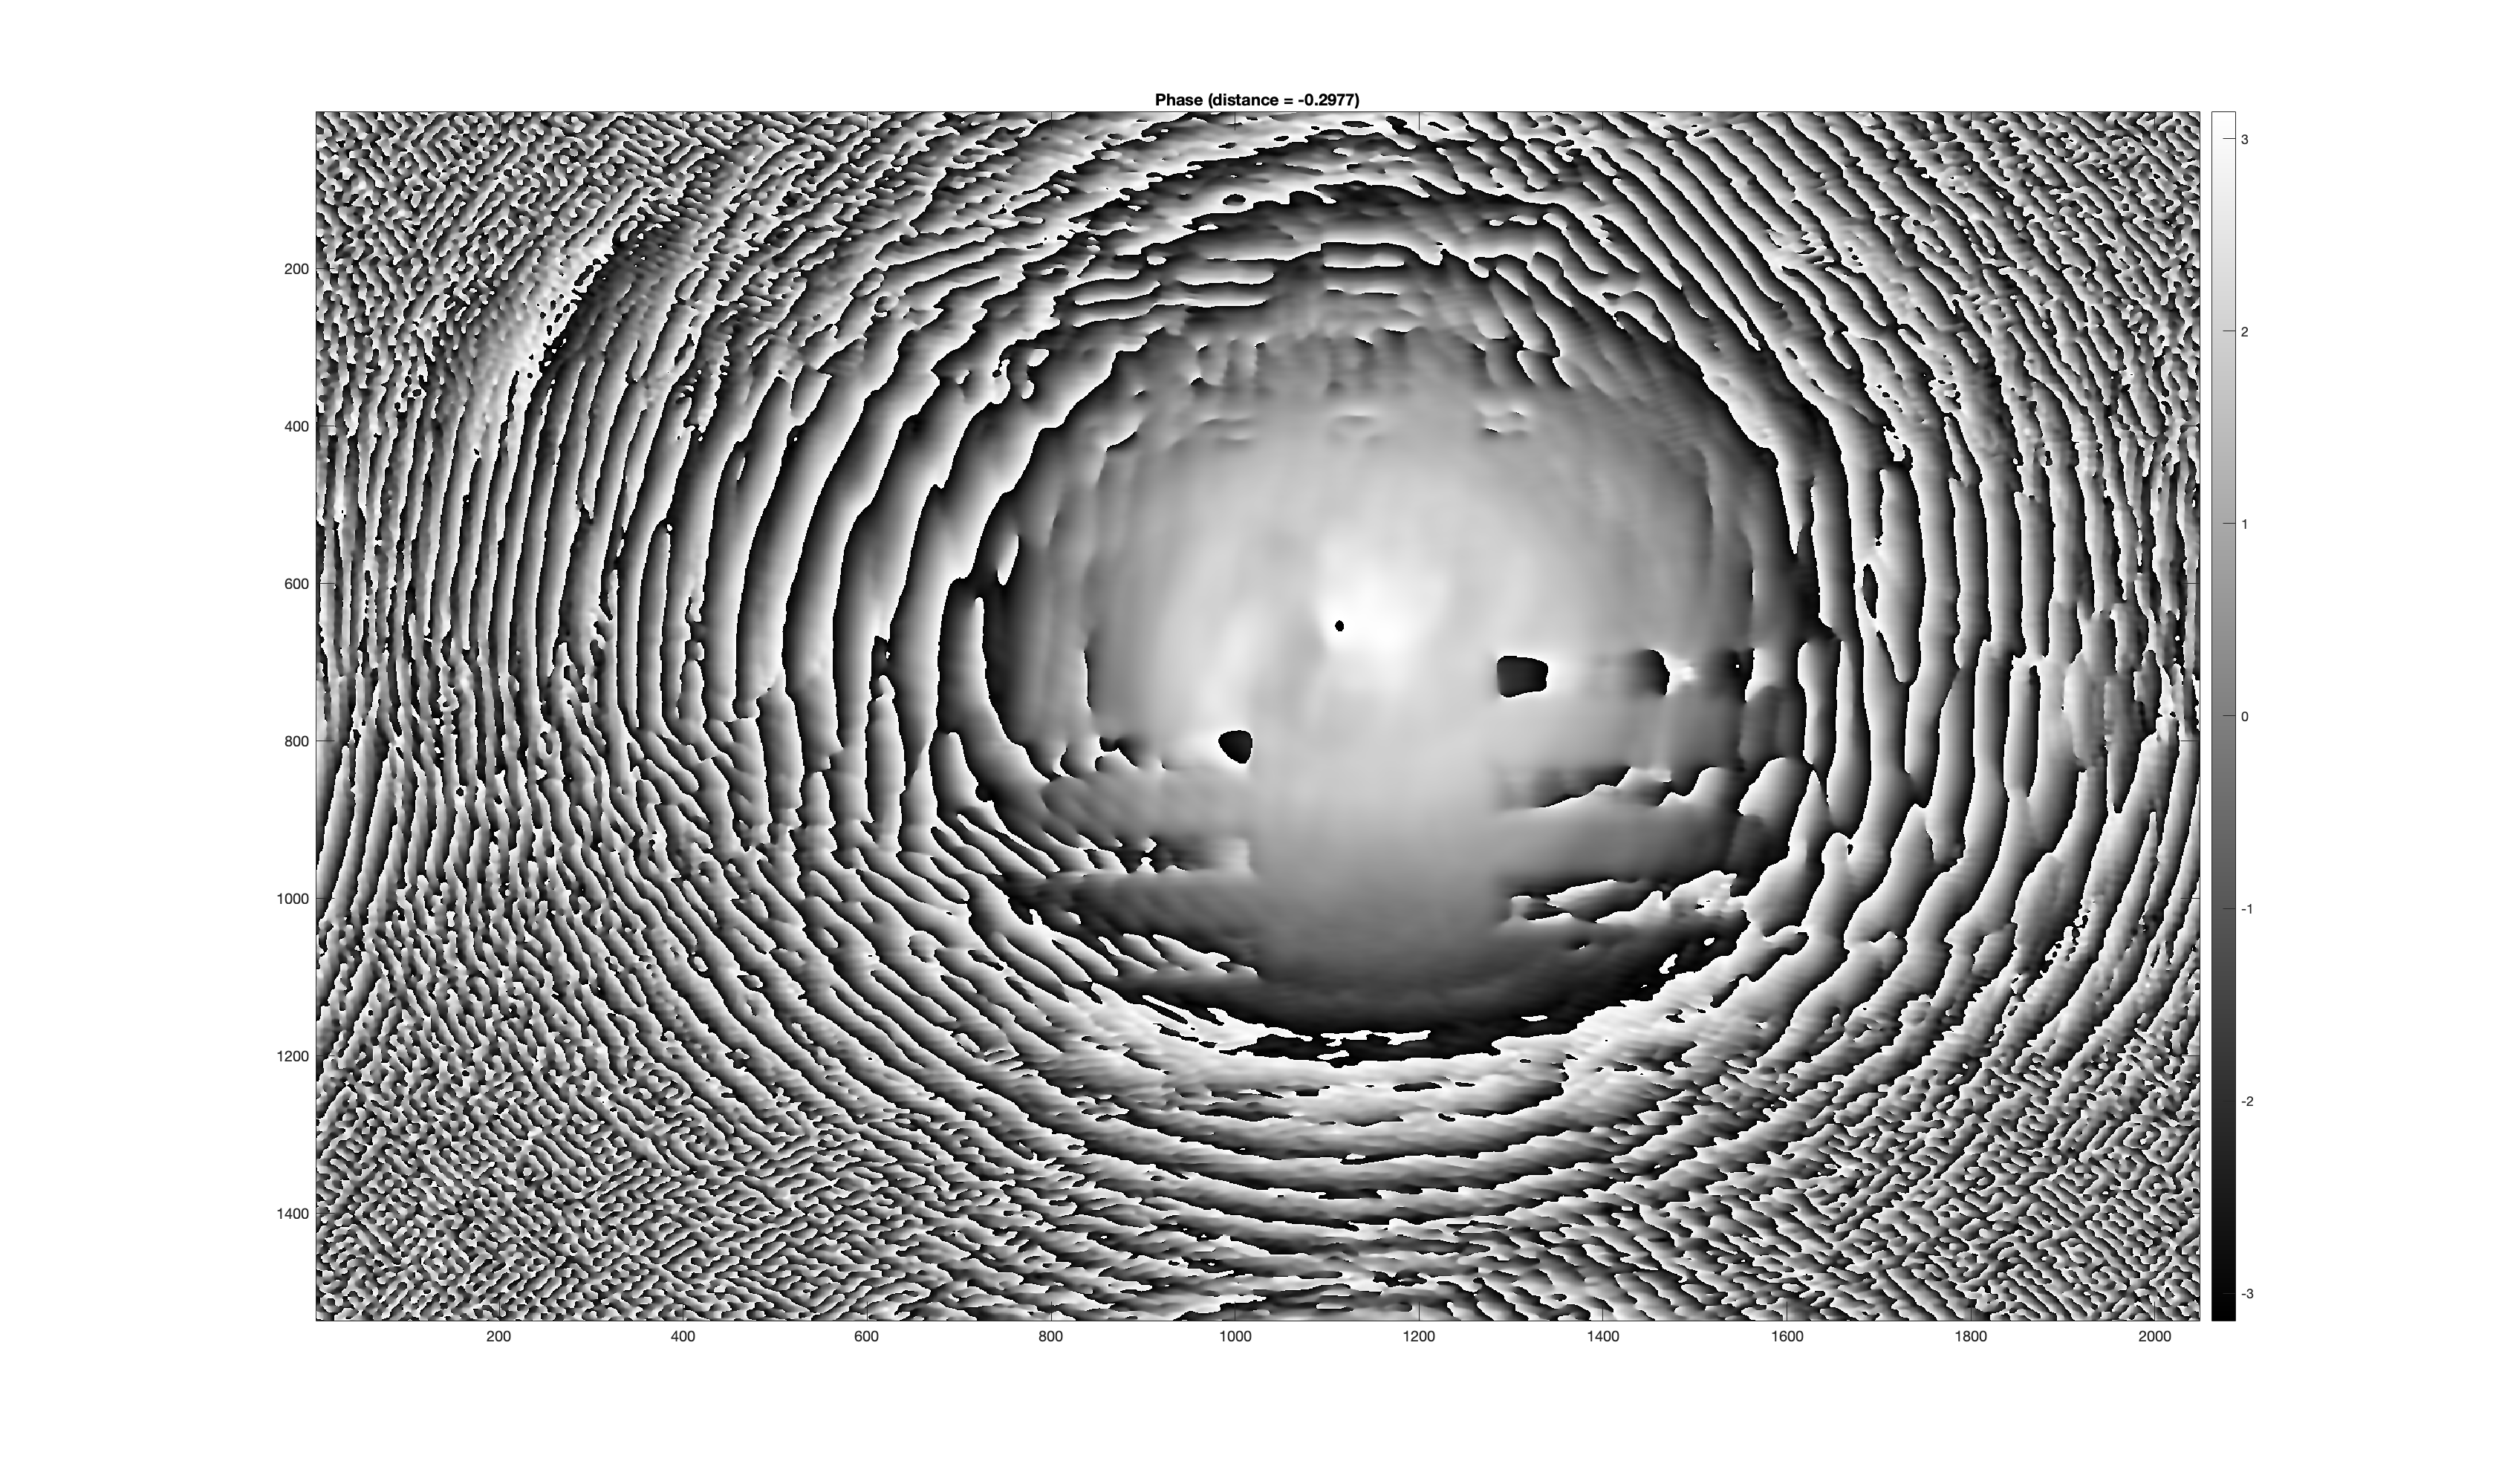
\includegraphics[width=\textheight]{img/5px_phase.png}
    }
    \caption{Phase of 5px image}
    \label{fig:my_label}
\end{figure}

\begin{figure}[p]
    \centering
    \rotatebox{270}{
        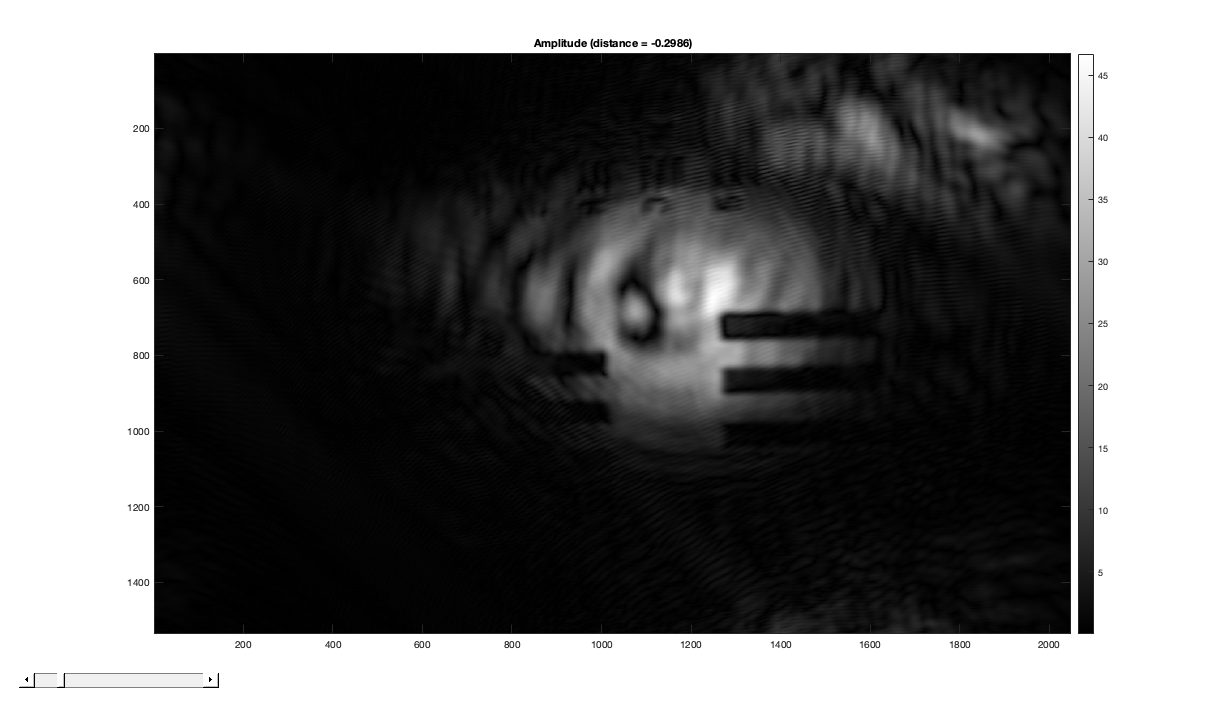
\includegraphics[width=\textheight]{img/12px_amplitude.png}
    }
    \caption{Amplitude of 12px image}
    \label{fig:my_label}
\end{figure}

\begin{figure}[p]
    \centering
    \rotatebox{270}{
        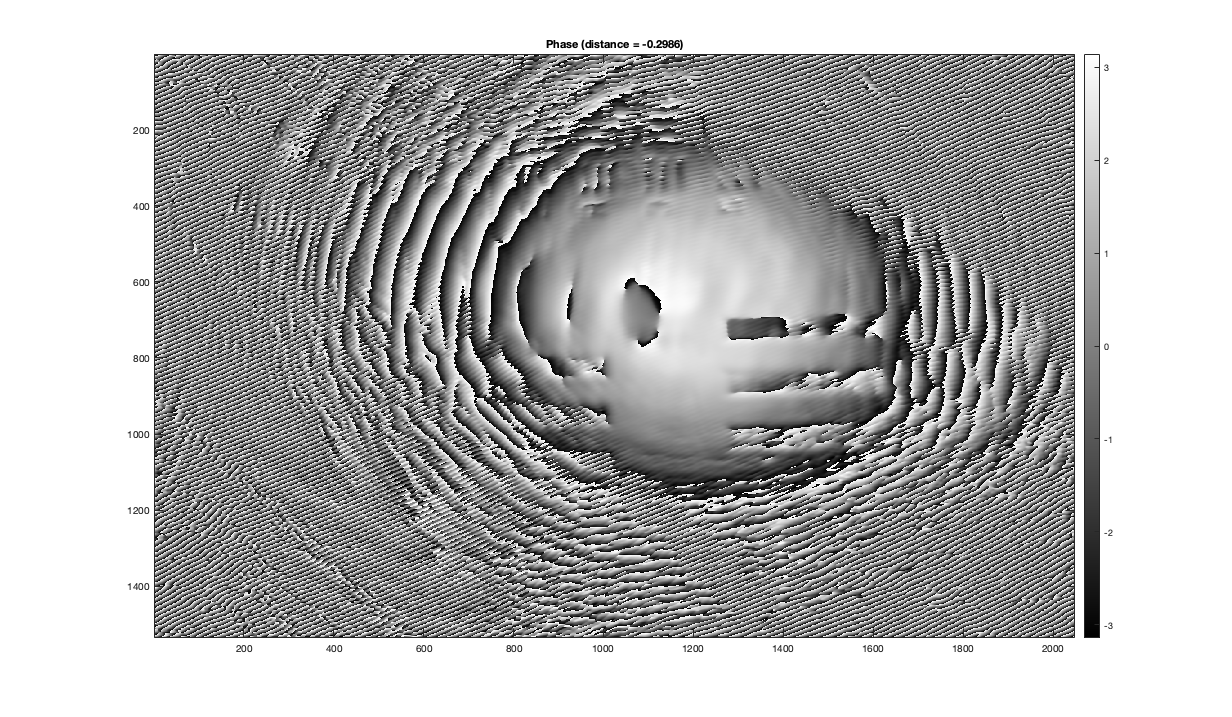
\includegraphics[width=\textheight]{img/12px_phase.png}
    }
    \caption{Phase of 12px image}
    \label{fig:my_label}
\end{figure}

\begin{figure}[p]
    \centering
    \rotatebox{270}{
        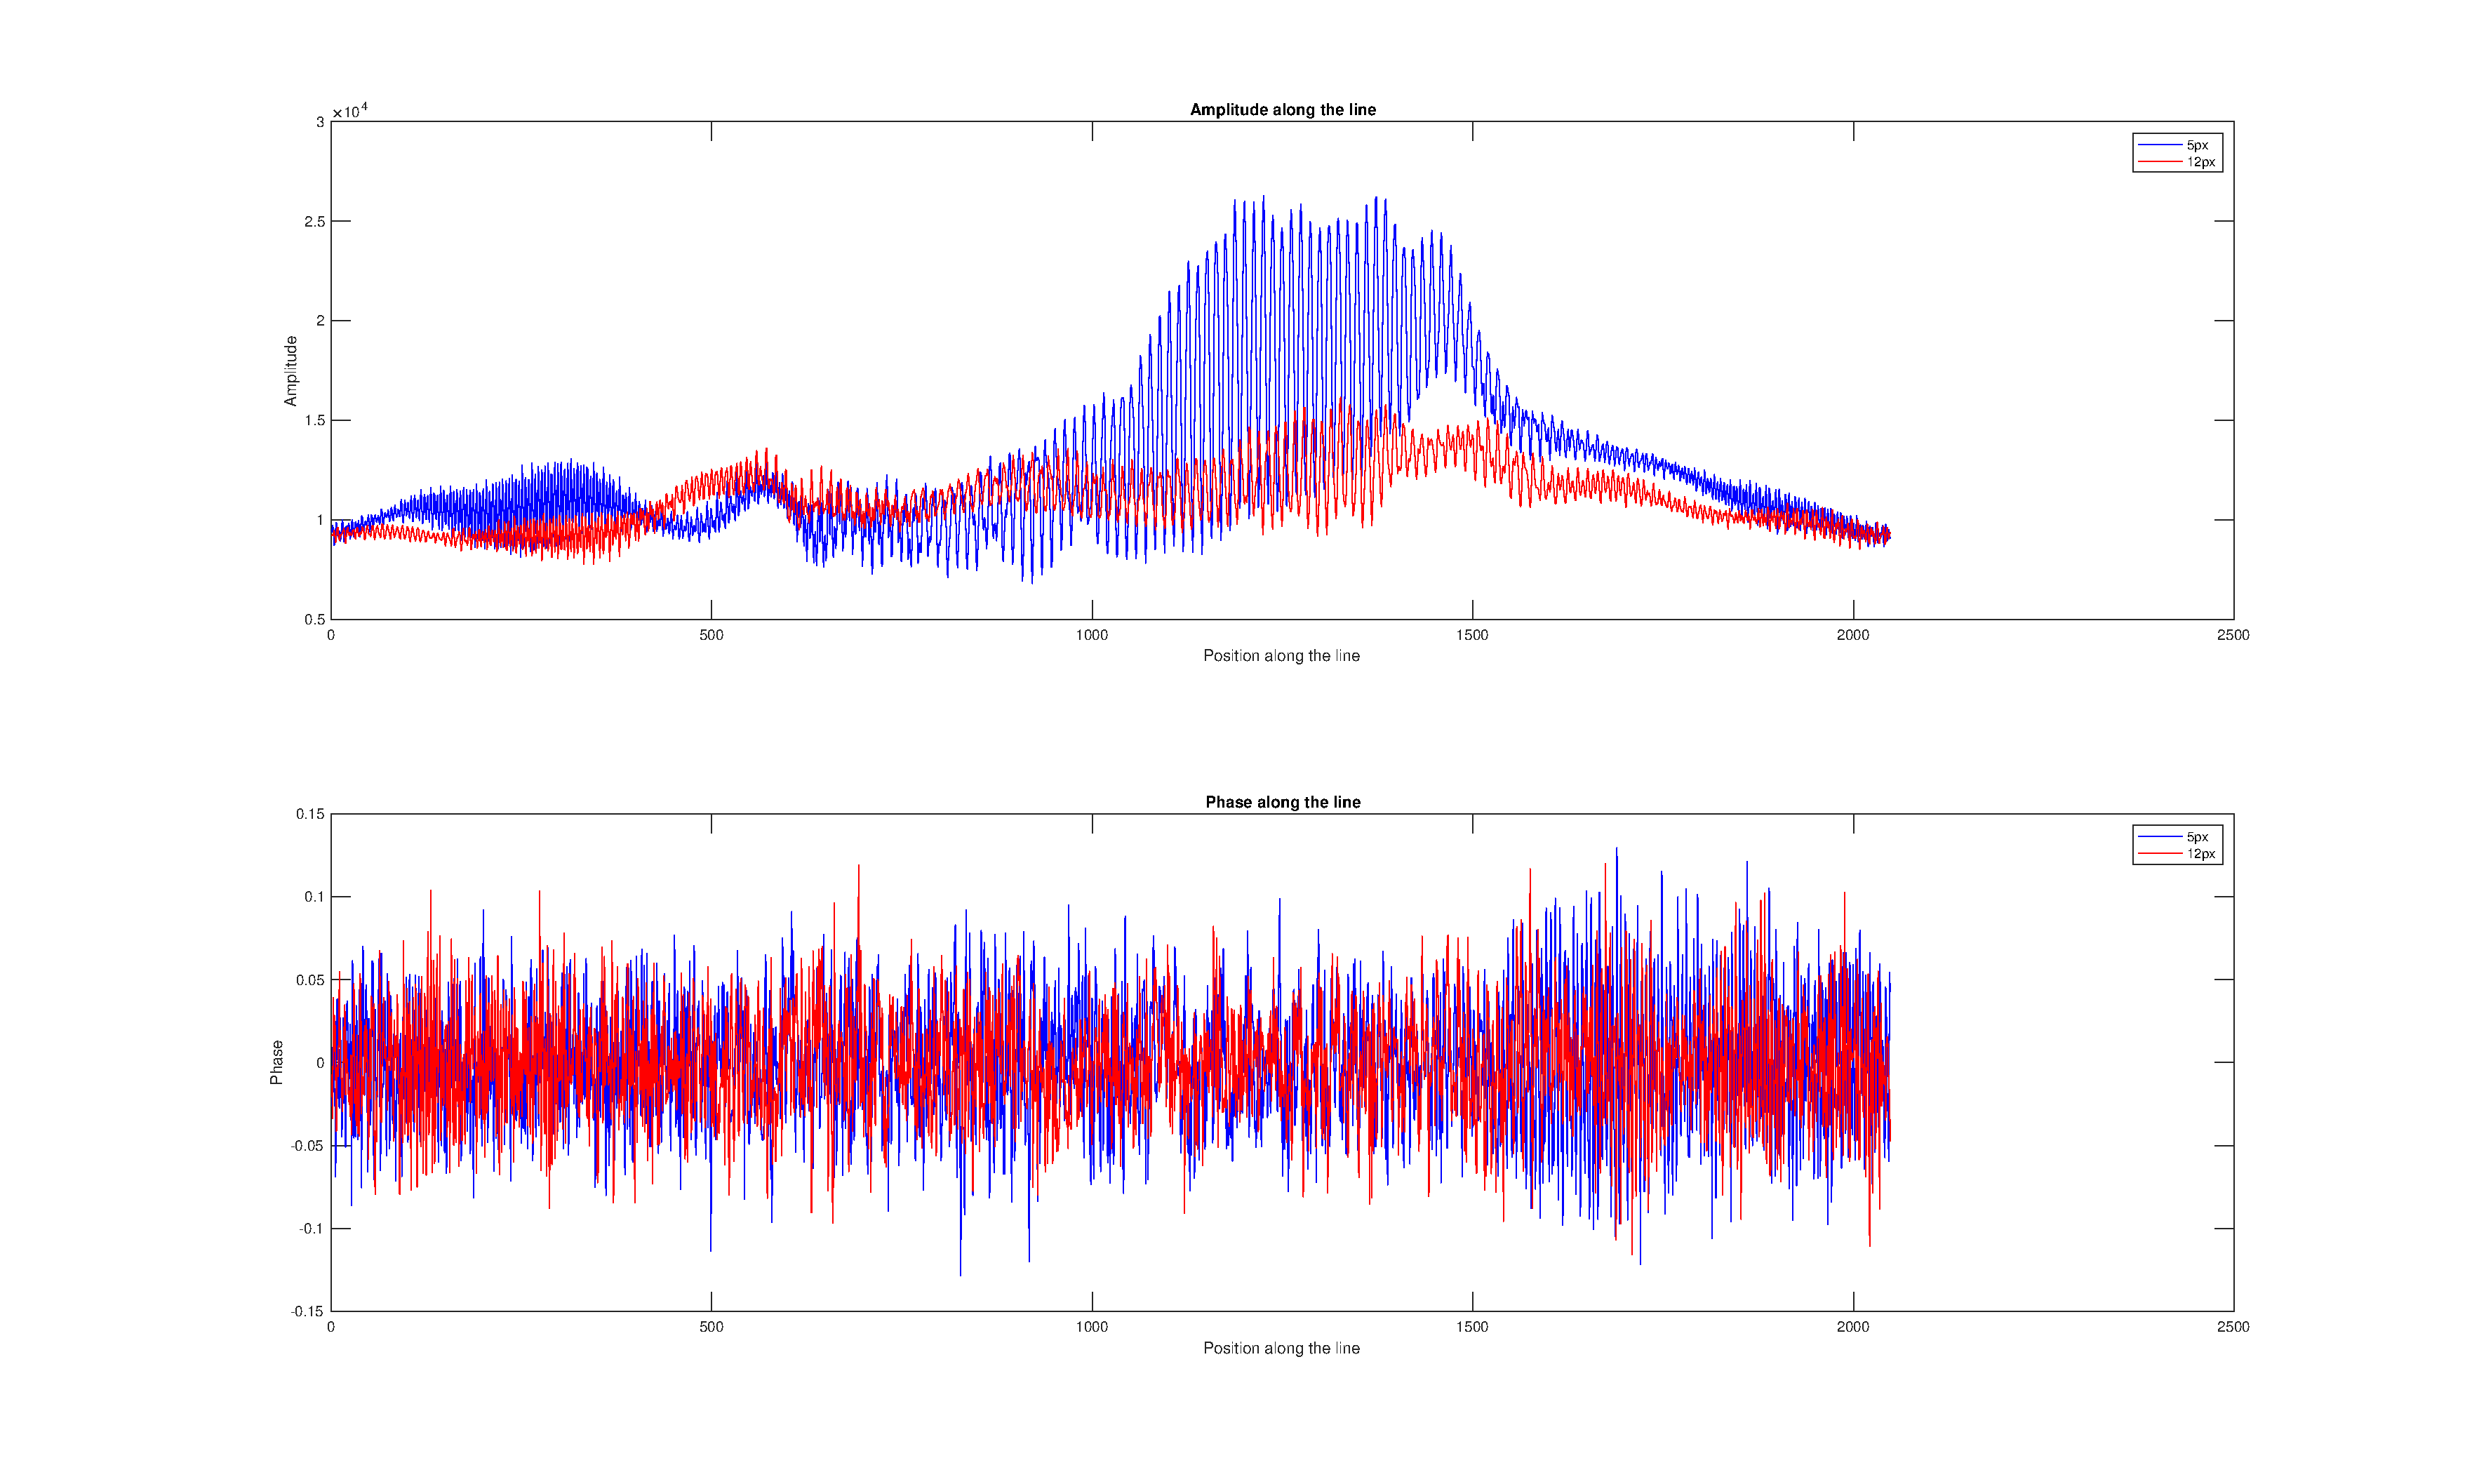
\includegraphics[width=\textheight]{img/lines.eps}
    }
    \caption{Mean amplitudes and phases between 5px and 12px wavefronts}
    \label{fig:my_label}
\end{figure}

\end{document}
